% Created 2016-05-24 二 22:38
\documentclass[xcolor=svgnames,presentation]{beamer}
\usepackage[utf8]{inputenc}
\usepackage[T1]{fontenc}
\usepackage{fixltx2e}
\usepackage{graphicx}
\usepackage{longtable}
\usepackage{float}
\usepackage{wrapfig}
\usepackage{soul}
\usepackage{textcomp}
\usepackage{marvosym}
\usepackage{wasysym}
\usepackage{latexsym}
\usepackage{amssymb}
\usepackage{hyperref}
\tolerance=1000
\usepackage{minted}
\usecolortheme[named=FireBrick]{structure}\setbeamercovered{transparent}\setbeamertemplate{caption}[numbered]\setbeamertemplate{blocks}[rounded][shadow=true] \usetheme{Darmstadt}\date{\today} \usepackage{tikz}\usepackage{xeCJK}\usepackage{amsmath}\setmainfont{Times New Roman}\setCJKmainfont[BoldFont={Adobe Heiti Std},ItalicFont={Adobe Fangsong Std}]{Adobe Heiti Std}\setCJKsansfont{Adobe Heiti Std}\setCJKmonofont{Adobe Fangsong Std}\usepackage{verbatim}\graphicspath{{figures/}} \definecolor{lstbgcolor}{rgb}{0.9,0.9,0.9} \usepackage{listings}\usepackage{minted} \usepackage{fancyvrb}\usepackage{xcolor}\lstset{escapeinside=`',frameround=ftft,language=C,breaklines=true,keywordstyle=\color{blue!70},commentstyle=\color{red!50!green!50!blue!50},frame=shadowbox,backgroundcolor=\color{yellow!20},rulesepcolor=\color{red!20!green!20!blue!20}}
\usemintedstyle{default}
\providecommand{\alert}[1]{\textbf{#1}}

\title{第9讲 DNS与DHCP服务配置管理}
\author{王晓庆}
\date{\today}
\hypersetup{
  pdfkeywords={},
  pdfsubject={},
  pdfcreator={Emacs Org-mode version 7.9.3f}}

\institute{wangxiaoqing@outlook.com}
\begin{document}

\maketitle

\begin{frame}
\frametitle{Outline}
\setcounter{tocdepth}{1}
\tableofcontents
\end{frame}
\section{DNS服务配置与管理}
\label{sec-1}
\begin{frame}[fragile]
\frametitle{Bind的安装与DNS服务器类型}
\label{sec-1-1}
\begin{itemize}

\item Bind的安装\\
\label{sec-1-1-1}%
\begin{minted}[]{bash}
rpm -qa | grep 'bind'
yum install bind bind-chroot bind-libs bind-utils
rpm -ql bind | less
\end{minted}

\item DNS服务器类型
\label{sec-1-1-2}%
\begin{enumerate}
\item 缓存服务器(Caching)
\item 转发服务器(Forwarding)
\item 主域名服务器(Master)
\item 从域名服务器(Slave)
\end{enumerate}
\end{itemize} % ends low level
\begin{block}{注意}
\label{sec-1-1-3}

一台服务器可以同时充当上述多种角色。
\end{block}
\end{frame}
\begin{frame}
\frametitle{实验环境搭建}
\label{sec-1-2}
\begin{itemize}

\item 实验拓扑图\\
\label{sec-1-2-1}%
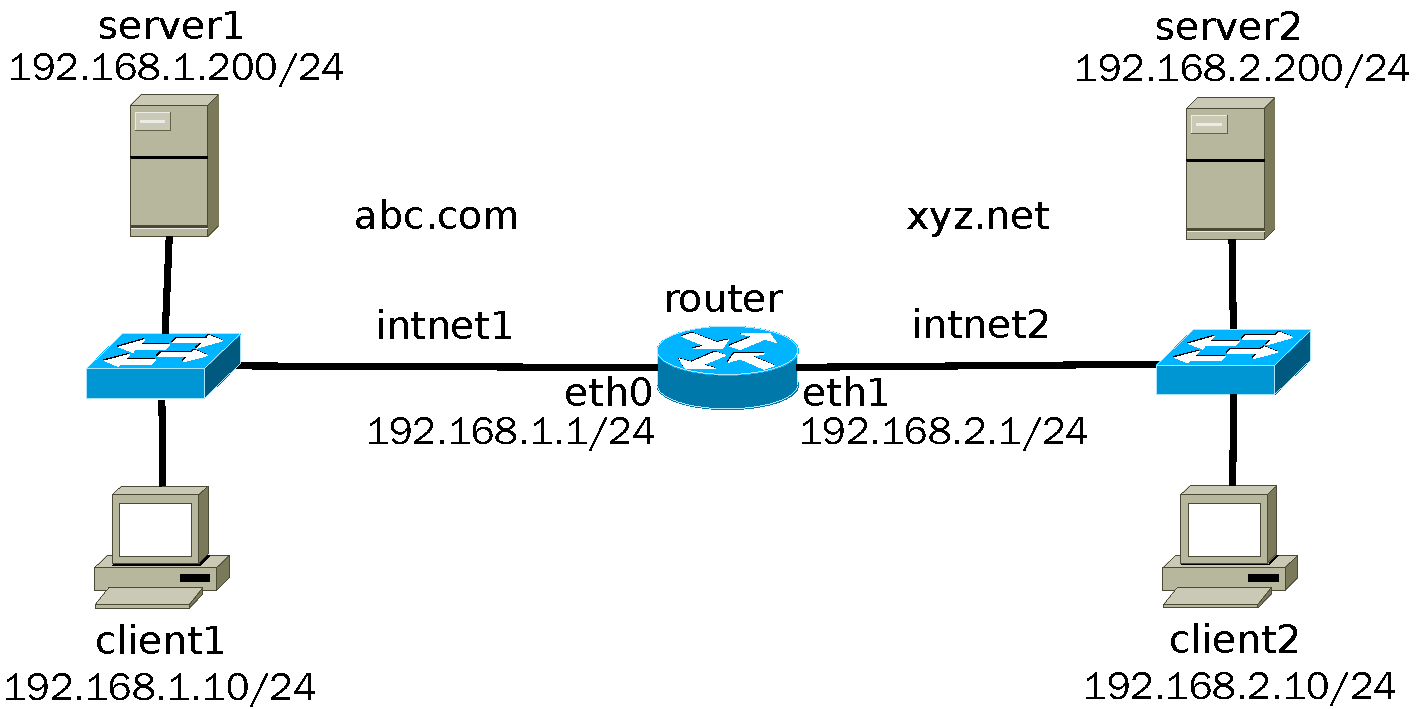
\includegraphics[width=.9\linewidth]{img/serverslab.pdf}

\item 实验准备
\label{sec-1-2-2}%
\begin{itemize}

\item 按图配置主机名、IP、默认网关等,保证所有主机能互相ping通。
\label{sec-1-2-2-1}%
\end{itemize} % ends low level
\end{itemize} % ends low level
\end{frame}
\begin{frame}[fragile]
\frametitle{缓存服务器的安装配置(server1)}
\label{sec-1-3}
\begin{itemize}

\item 默认情况下bind并未提供主配置文件
\label{sec-1-3-1}%
\begin{itemize}

\item /var/named/chroot/etc/named.conf
\label{sec-1-3-1-1}%
\end{itemize} % ends low level

\item 安装缓存服务器\\
\label{sec-1-3-2}%
\begin{minted}[]{bash}
yum -y install caching-nameserver
rpm -ql caching-nameserver
service named start
\end{minted}
\end{itemize} % ends low level
\end{frame}
\begin{frame}[fragile]
\frametitle{缓存服务器的默认配置}
\label{sec-1-4}


\begin{minted}[]{bash}
cd /var/named/chroot/etc
grep -v '//' named.caching-nameserver.conf
options {
        listen-on port 53 { 127.0.0.1; }; #仅监听环回接口
        listen-on-v6 port 53 { ::1; };
        directory       "/var/named"; #指定默认工作目录
        dump-file       "/var/named/data/cache_dump.db";
        statistics-file "/var/named/data/named_stats.txt";
        memstatistics-file "/var/named/data/named_mem_stats.txt";
        allow-query     { localhost; }; #仅允许本机访问
        allow-query-cache { localhost; }; #本机访问缓存
};
\end{minted}
\end{frame}
\begin{frame}[fragile]
\frametitle{缓存服务器的默认配置(2)}
\label{sec-1-5}


\begin{minted}[]{bash}
logging {
        channel default_debug { #定义日志通道
                file "data/named.run"; #默认日志文件
                severity dynamic; #默认日志等级
        };
};
view localhost_resolver { #定义视图
        match-clients      { localhost; }; #匹配请求源地址
        match-destinations { localhost; }; #匹配请求目标地址
        recursion yes; #允许递归查询
        include "/etc/named.rfc1912.zones"; #包含区域文件
};
\end{minted}
\end{frame}
\begin{frame}[fragile]
\frametitle{修改缓存服务器默认配置}
\label{sec-1-6}


\begin{minted}[]{bash}
vim named.caching-nameserver.conf
acl corpnets { 192.168.1.0/24; 192.168.2.0/24; };
options {
        listen-on port 53 { any; }; #监听所有接口
        directory "/var/named";
        allow-query { corpnets; }; #允许指定客户端
        recursion yes; #允许递归查询
};
include "/etc/named.rfc1912.zones"; #包含区域文件

service named restart #重启named服务使配置生效
cat /var/named/chroot/etc/named.rfc1912.zones
ls /var/named/chroot/var/named #查看区域文件所在目录
\end{minted}
\end{frame}
\begin{frame}[fragile]
\frametitle{配置主域名服务器(server1)(1)}
\label{sec-1-7}
\begin{itemize}

\item 1. 配置named.conf文件,添加区域\\
\label{sec-1-7-1}%
\begin{minted}[]{bash}
cd /var/named/chroot/etc
cp -p named.caching-nameserver.conf named.conf
vim named.conf #在最后添加下面几行
zone "abc.com" IN {
        type master;
        file "abc.com.zone";
};
zone "1.168.192.in-addr.arpa" IN {
        type master;
        file "192.168.1.rev";
};
\end{minted}
\end{itemize} % ends low level
\end{frame}
\begin{frame}[fragile]
\frametitle{配置主域名服务器(server1)(2)}
\label{sec-1-8}
\begin{itemize}

\item 2. 创建正向区域文件abc.com.zone\\
\label{sec-1-8-1}%
\begin{minted}[]{bash}
cp -p localhost.zone abc.com.zone
vim abc.com.zone
$TTL 86400
@       IN SOA ns1.abc.com. root.abc.com. (
                                42   ; serial
                                3H   ; refresh
                                15M  ; retry
                                1W   ; expiry
                                1D ) ; minimum
        IN NS           ns1.abc.com.
        IN MX    5      mail.abc.com.
ns1     IN A            192.168.1.200
www     IN A            192.168.1.200
ftp     IN CNAME        www.abc.com.
mail    IN A            192.168.1.200
\end{minted}
\end{itemize} % ends low level
\end{frame}
\begin{frame}[fragile]
\frametitle{配置主域名服务器(server1)(3)}
\label{sec-1-9}
\begin{itemize}

\item 3. 创建反向区域文件192.168.1.rev\\
\label{sec-1-9-1}%
\begin{minted}[]{bash}
cp -p named.local 192.168.1.rev
vim 192.168.1.rev
$TTL 86400
@ IN SOA ns1.abc.com. root.abc.com. (
                         2016052001 ; Serial
                         28800      ; Refresh
                         14400      ; Retry
                         3600000    ; Expire
                         86400 )    ; Minimum
        IN      NS      ns1.abc.com.
200     IN      PTR     ns1.abc.com.
200     IN      PTR     www.abc.com.
200     IN      PTR     ftp.abc.com.
200     IN      PTR     mail.abc.com.
10      IN      PTR     client1.abc.com.
\end{minted}
\end{itemize} % ends low level
\end{frame}
\begin{frame}[fragile]
\frametitle{配置主域名服务器(server1)(4)}
\label{sec-1-10}
\begin{itemize}

\item 检查配置文件\\
\label{sec-1-10-1}%
\begin{minted}[]{bash}
cd /var/named/chroot/etc
named-checkconf named.conf #检查主配置文件
cd /var/named/chroot/var/named
named-checkzone abc.com abc.com.zone #检查区域文件
named-checkzone 1.168.192.in-addr.arpa 192.168.1.rev
\end{minted}

\item 重启named服务,使配置生效\\
\label{sec-1-10-2}%
\begin{minted}[]{bash}
service named restart
\end{minted}
\end{itemize} % ends low level
\end{frame}
\begin{frame}[fragile]
\frametitle{客户端配置及测试(client1)}
\label{sec-1-11}
\begin{itemize}

\item 客户端配置\\
\label{sec-1-11-1}%
\begin{minted}[]{bash}
vim /etc/resolv.conf
nameserver 192.168.1.200
\end{minted}

\item 客户端测试\\
\label{sec-1-11-2}%
\begin{minted}[]{bash}
host [-t type] domain-name [dns-server]
host www.abc.com [192.168.1.200]
host -t mx abc.com [192.168.1.200]
nslookup ftp.abc.com [192.168.1.200]
nslookup [- 192.168.1.200] #开始交互查询
set type=mx
abc.com
exit                       #退出交互查询
dig @server domain type
dig @192.168.1.200 abc.com ns
\end{minted}
\end{itemize} % ends low level
\end{frame}
\begin{frame}[fragile]
\frametitle{配置从域名服务器(server1)(1)}
\label{sec-1-12}
\begin{itemize}

\item 1. 编辑主域名服务器主配置文件\\
\label{sec-1-12-1}%
\begin{minted}[]{bash}
cd /var/named/chroot/etc
vim named.conf #添加allow-transfer语句
zone "abc.com" IN {
        type master;
        file "abc.com.zone";
        allow-transfer { 192.168.2.200; };
};
zone "1.168.192.in-addr.arpa" IN {
        type master;
        file "192.168.1.rev";
        allow-transfer { 192.168.2.200; };
};
\end{minted}
\end{itemize} % ends low level
\end{frame}
\begin{frame}[fragile]
\frametitle{配置从域名服务器(server2)(2)}
\label{sec-1-13}
\begin{itemize}

\item 2. 编辑从域名服务器主配置文件\\
\label{sec-1-13-1}%
\begin{minted}[]{bash}
cd /var/named/chroot/etc
scp root@192.168.1.200:/var/named/chroot\
/etc/named.conf .
chgrp named named.conf #将配置文件归属named组
vim named.conf #修改区域定义相关内容
zone "abc.com" IN {
        type slave;
        file "slaves/abc.com.zone";
        masters { 192.168.1.200; };
};
zone "1.168.192.in-addr.arpa" IN {
        type slave;
        file "slaves/192.168.1.rev";
        masters { 192.168.1.200; };
};
\end{minted}
\end{itemize} % ends low level
\end{frame}
\begin{frame}[fragile]
\frametitle{配置从域名服务器(server1和server2)}
\label{sec-1-14}
\begin{itemize}

\item 3. 使配置生效并检查、测试从域名服务器\\
\label{sec-1-14-1}%
\begin{minted}[]{bash}
cd /var/named/chroot/var/named
ls slaves
#重启server1的named服务
service named restart
#重启server2的named服务
service named restart
ls slaves
\end{minted}
\end{itemize} % ends low level
\begin{block}{注意}
\label{sec-1-14-2}

每次修改主域名服务器的区域文件后,一定不要忘记增加其SOA记录中的序号,否则从域名服务器将得不到区域更新!
\end{block}
\begin{itemize}

\item 4. 客户端测试(略)
\label{sec-1-14-3}%
\end{itemize} % ends low level
\end{frame}
\begin{frame}
\frametitle{练习}
\label{sec-1-15}
\begin{itemize}

\item 在server2上配置xyz.net域的主域名服务器
\label{sec-1-15-1}%
\begin{enumerate}
\item 编辑named.conf文件
\item 编辑xyz.net.zone正向区域文件
\item 编辑192.168.2.rev反向区域文件
\item 检查配置文件和区域文件
\item 重启named服务
\item 配置dns客户端(client2)
\item 客户端测试
\end{enumerate}
\end{itemize} % ends low level
\end{frame}
\begin{frame}[fragile]
\frametitle{配置区域委派(1)}
\label{sec-1-16}
\begin{itemize}

\item 1. 在子域主域名服务器(server2)上配置子域\\
\label{sec-1-16-1}%
\begin{minted}[]{bash}
cd /var/named/chroot
vim etc/named.conf #在最后面添加子域定义
zone "jx.abc.com" IN {
  type master;
  file "jx.abc.com.zone";
};
#此处不需要重复定义反向区域2.168.192.in-addr.arpa
\end{minted}
\end{itemize} % ends low level
\end{frame}
\begin{frame}[fragile]
\frametitle{配置区域委派(2)}
\label{sec-1-17}
\begin{itemize}

\item 2. 在子域主域名服务器(server2)上配置子域正向区域文件\\
\label{sec-1-17-1}%
\begin{minted}[]{bash}
vim var/named/jx.abc.com.zone
$TTL 86400
@       IN      SOA ns1  root (
                                42   ; serial
                                3H   ; refresh
                                15M  ; retry
                                1W   ; expiry
                                1D ) ; minimum
        IN NS           ns1.jx.abc.com.
ns1     IN A            192.168.2.200
www     IN A            192.168.2.200
ftp     IN CNAME        www.abc.com.
\end{minted}
\end{itemize} % ends low level
\end{frame}
\begin{frame}[fragile]
\frametitle{配置区域委派(3)}
\label{sec-1-18}
\begin{itemize}

\item 3. 在子域主域名服务器(server2)上配置子域反向区域文件\\
\label{sec-1-18-1}%
\begin{minted}[]{bash}
vim var/named/192.168.2.rev #在最后面添加几行记录
        IN      NS      ns1.jx.abc.com.
200     IN      PTR     ns1.jx.abc.com.
200     IN      PTR     www.jx.abc.com.
200     IN      PTR     ftp.jx.abc.com.
\end{minted}
\end{itemize} % ends low level
\end{frame}
\begin{frame}[fragile]
\frametitle{配置区域委派(4)}
\label{sec-1-19}
\begin{itemize}

\item 4. 在父域域名服务器(server1)正向区域文件中上添加委派记录\\
\label{sec-1-19-1}%
\begin{minted}[]{bash}
cd /var/named/chroot/var/named
vim abc.com.zone   #在最后面添加子域委派记录
jx      IN      NS      ns1.jx.abc.com.
ns1.jx  IN      A       192.168.2.200
\end{minted}

\item 5. 重启父域和子域named服务\\
\label{sec-1-19-2}%
\begin{minted}[]{bash}
service named restart
\end{minted}

\item 6. 客户端测试
\label{sec-1-19-3}%
\begin{itemize}

\item 通过父域域名服务器查询得到的是非权威答案\\
\label{sec-1-19-3-1}%
\begin{minted}[]{bash}
nslookup ftp.jx.abc.com 192.168.1.200
\end{minted}
\end{itemize} % ends low level
\end{itemize} % ends low level
\end{frame}
\begin{frame}[fragile]
\frametitle{配置转发器(1)}
\label{sec-1-20}
\begin{itemize}

\item 在server1上配置全局转发\\
\label{sec-1-20-1}%
\begin{minted}[]{bash}
host ftp.xyz.net 192.168.1.200 #无法解析!
cd /var/named/chroot/etc
vim named.conf #添加下面几行
options {
        listen-on port 53 { any; };
        directory       "/var/named";
  forward only; #仅转发,也可为first(先转发)
  forwarders { 192.168.2.200; }; #配置转发器
        allow-query     { any; };
        recursion yes;
};

service named restart #重启named服务
host ftp.xyz.net 192.168.1.200 #解析成功!
\end{minted}
\end{itemize} % ends low level
\end{frame}
\begin{frame}[fragile]
\frametitle{配置转发器(2)}
\label{sec-1-21}
\begin{itemize}

\item 在server1上配置区域转发\\
\label{sec-1-21-1}%
\begin{minted}[]{bash}
cd /var/named/etc
vim named.conf #修改主配置文件
options {
        listen-on port 53 { any; };
        directory       "/var/named";
        allow-query     { any; };
        recursion yes;
};
...
zone "xyz.net" IN {  #添加转发区域
  type forward;
  forwarders: { 192.168.2.200; };
};
\end{minted}
\end{itemize} % ends low level
\end{frame}
\section{DHCP服务配置与管理}
\label{sec-2}
\begin{frame}[fragile]
\frametitle{在server1上安装配置dhcp服务器(1)}
\label{sec-2-1}
\begin{itemize}

\item 1. 安装dhcp服务\\
\label{sec-2-1-1}%
\begin{minted}[]{bash}
rpm -qa | grep dhcp
yum install dhcp
rpm -ql dhcp
\end{minted}
\end{itemize} % ends low level
\end{frame}
\begin{frame}[fragile]
\frametitle{在server1上安装配置dhcp服务器(2)}
\label{sec-2-2}
\begin{itemize}

\item 2. 配置dhcp服务\\
\label{sec-2-2-1}%
\begin{minted}[]{bash}
cd /usr/share/doc/dhcp-3.0.5/
cp dhcpd.conf.sample /etc/dhcpd.conf
vim dhcpd.conf
ddns-update-style interim;
ignore client-updates;
subnet 192.168.1.0 netmask 255.255.255.0 {
        option routers                  192.168.1.1;
        option subnet-mask              255.255.255.0;
        option domain-name-servers      192.168.1.200;
        range 192.168.1.50 192.168.1.199;
        default-lease-time 21600;
        max-lease-time 43200;
}
\end{minted}
\end{itemize} % ends low level
\end{frame}
\begin{frame}[fragile]
\frametitle{在server1上安装配置dhcp服务器(3)}
\label{sec-2-3}
\begin{itemize}

\item 3. 测试dhcp服务器
\label{sec-2-3-1}%
\begin{itemize}

\item 启动dhcpd服务\\
\label{sec-2-3-1-1}%
\begin{minted}[]{bash}
chkconfig --level 3 dhcpd on
service dhcpd start
\end{minted}

\item 配置dhcp客户端client1\\
\label{sec-2-3-1-2}%
\begin{minted}[]{bash}
cd /etc/sysconfig/network-scripts
vim ifcfg-eth1
DEVICE=eth1
BOOTPROTO=dhcp
ONBOOT=yes

dhclient   #启动dhcp客户端
ifconfig
cat /var/lib/dhclient/dhclient.leases #client1上查看租约
cat /var/lib/dhcpd/dhcpd.leases #server1上查看租约
\end{minted}
\end{itemize} % ends low level
\end{itemize} % ends low level
\end{frame}
\begin{frame}[fragile]
\frametitle{安装配置dhcp中继代理(1)}
\label{sec-2-4}
\begin{itemize}

\item 1. 配置dhcp服务器server1\\
\label{sec-2-4-1}%
\begin{minted}[]{bash}
vim /etc/dhcpd.conf  #在最后面添加子网
subnet 192.168.2.0 netmask 255.255.255.0 {
        option routers                  192.168.2.1;
        option subnet-mask              255.255.255.0;
        option domain-name-servers      192.168.2.200;
        range 192.168.2.50 192.168.2.199;
        default-lease-time 21600;
        max-lease-time 43200;
}
\end{minted}
\end{itemize} % ends low level
\end{frame}
\begin{frame}[fragile]
\frametitle{安装配置dhcp中继代理(2)}
\label{sec-2-5}
\begin{itemize}

\item 2. 配置dhcp中继代理server2\\
\label{sec-2-5-1}%
\begin{minted}[]{bash}
yum install dhcp
chkconfig --level 3 dhrelay on
vim /etc/sysconfig/dhcrelay
DHCRELAYARGS="" #运行参数
INTERFACES=""   #监听接口,如"eth0 eth1"
DHCPSERVERS="192.168.2.200" #指定dhcp服务器
#注意:dhcp中继代理本身必须有静态地址并能与服务器通信
service dhrelay start
\end{minted}
\end{itemize} % ends low level
\end{frame}
\begin{frame}[fragile]
\frametitle{安装配置dhcp中继代理(3)}
\label{sec-2-6}
\begin{itemize}

\item 3. 配置dhcp客户端client2\\
\label{sec-2-6-1}%
\begin{minted}[]{bash}
cd /etc/sysconfig/network-scripts
vim ifcfg-eth1
DEVICE=eth1
BOOTPROTO=dhcp
ONBOOT=yes

dhclient   #启动dhcp客户端
ifconfig
cat /var/lib/dhclient/dhclient.leases #client2上查看租约
cat /var/lib/dhcpd/dhcpd.leases #server1上查看租约
\end{minted}
\end{itemize} % ends low level
\end{frame}

\end{document}
